 \subsection{Kvantitativní -- Numerická proměnná}
\begin{itemize}
	\item \textbf{Míry polohy} --  určující typické rozložení hodnot proměnné (jejich rozmístění na číselné ose).

 		\begin{itemize}
 			\item Průměr -- $\bar{x} = \frac{\sum\limits_{i=1}^n x_i}{n}$
 			\item Modus -- střed shorthu
 			\item Kvantily -- dolní kvartil, médián, horní kvartil,..
 		\end{itemize}
 	\item \textbf{Míry variability} -- určující variabilitu (rozptyl) hodnot kolem své typické polohy.
 		\begin{itemize}
 			\item Variační rozpětí $x_{max} - x_{min}$
 			\item Inverkvartilové rozpětí -- $IQR = x_{0,75} - x_{0,25}$
 			\item Výběrový rozptyl
 			\item Výběrová směrodatná odchylka
 			\item Variační koeficient
 		\end{itemize}
 	\item \textbf{Míra šikmosti a špičatosti}	
 		\begin{itemize}
 			\item Výběrová šikmost
 			\item Výběrová špičatost
 		\end{itemize}
 	\item \textbf{Identifikace odlehlých pozorování}	
 		\begin{itemize}
 			\item Vnitřní hradby dolní mez: $h_D = x_{0,25} - 1,5IQR$, horní mez: $h_H = x_{0,75} + 1,5IQR$
 			\item Vnější hradby dolní mez: $h_D = x_{0,25} - 3IQR$, horní mez: $h_H = x_{0,75} + 3IQR$
 			\item Z--souřadnice
 			\item Mediánová souřadnice
 		\end{itemize}
\end{itemize}

\textbf{Grafické zobrazení numerické proměnné:}
\begin{itemize}
	\item Empirická distribuční funkce
	\item Krabicový graf (box plot)
	\item Číslicový histogram (lodyha s listy, steam and leaf)
\end{itemize}

 \subsection{Kvalitativní --Kategoriální proměnná}
\begin{enumerate}[label=\alph*)]
	\item Nominální proměnná -- nemá smysl uspořádaní
	\begin{itemize}
		\item \textbf{Základní statistiky pro popis nominální proměnné:}
	 		\begin{itemize}
	 			\item četnost
	 			\item relativní četnost
	 			\item modus
	 		\end{itemize}
	\item \textbf{Grafické zobrazení nominální proměnné:}
			\begin{itemize}
				\item histogram
				\item výsečový graf
			\end{itemize}
	\end{itemize}
	\item Ordinální proměnná -- má smysl uspořádání
	\begin{itemize}
		\item \textbf{Základní statistiky pro popis ordinální proměnné:}
	 		\begin{itemize}
	 			\item četnost
	 			\item relativní četnost
	 			\item kumulativní četnost
	 			\item relativní kumulativní četnost
	 			\item modus
	 		\end{itemize}
		\item \textbf{Grafické zobrazení ordinální proměnné:}
				\begin{itemize}
						\item histogram
						\item výsečový graf
						\item Lorenzova křivka
						\item Paretův graf
				\end{itemize}
	\end{itemize}
\end{enumerate}
\textbf{Paretův princip} – 80\% následků pramení z 20\% příčin.\\
\textbf{Paretova analýza} – postup vedoucí k nalezení \uv{životně důležité menšiny} (spektra příčin ovlivňujících rozhodujícím způsobem následky).


\subsection{Míry polohy a variability}
Snad nejpoužívanějšími mírami polohy jsou průměry proměnných. Průměry představují průměrnou nebo typickou hodnotu výběrového souboru. Zřejmě nejznámějším průměrem pro kvantitativní proměnnou je \textbf{aritmetický průměr}
\begin{itemize}
	\item \textbf{Aritmetický průměr} $\mathbf{\bar{x}}$ (mean)
	\item \textbf{Aritmetický vážený průměr}
	\item \textbf{Harmonický průměr}  -- Pro výpočet průměru v případech, kdy proměnná má charakter části z celku (úlohy o společné práci, ...).
	\item \textbf{Harmonický vážený průměr} -- Pokud máme údaje setříděné do tabulky četností.
	\item \textbf{Geometrický průměr} -- Pracujeme-li s kladnou proměnnou představující relativní změny (růstové indexy,cenové indexy...). $\bar{x}_G = \sqrt[n]{x_1 \cdot x_2 \cdot ... \cdot x_n}$
	\item \textbf{Geometrický vážený průměr} -- Pracujeme-li s kladnou proměnnou představující relativní změny (růstové indexy,cenové indexy...). $\bar{x}_G = \sqrt[n]{x_1^{n_1} \cdot x_2^{n_2} \cdot ... \cdot x_n^{n_k}}$ kde $n = \sum\limits_{i=1}^k n_i$. \\

	\item \textbf{Modus} -- Pro \textbf{diskrétní proměnnou} definujeme modus jako hodnotu nejčetnější varianty proměnné (podobně jako u kvalitativní proměnné), u spojité proměnné považujeme za modus $\mathbf{\hat{x}}$ hodnotu kolem níž je největší koncentrace hodnot proměnné. Mnohdy mluvíme o typické hodnotě proměnné. Pro určení této hodnoty využijeme tzv. \textbf{short}, což je nejkratší interval, v němž leží alespoň 50\% hodnot proměnné (v případě výběru o rozsahu $n = 2k(k \in N)$ (sudý počet hodnot), leží v shorthu $k$ hodnotě - což je 50\% $(n/2)$ hodnot proměnné, v případě výběru o rozsahu $n = 2k + 1(k \in N)$ (lichý počet hodnot), leží v shorthu $k + 1$ hodnot - což je o 1 více než je 50\% hodnot proměnné). \textbf{Modus pak definujeme jako střed shorthu}. \\

	\item \textbf{Výběrové kvantily} (quantile, resp. percentile) -- jsou to statistiky, které charakterizují polohu jednotlivých hodnot v rámci proměnné. Podobně jako modus, jsou i výběrové kvantily \textbf{rezistentní} (odolné) vůči odlehlým pozorováním. Obecně je výběrový kvantil chápán jako hodnota, která rozděluje výběrový soubor na dvě části -- hodnoty, které jsou menší než daný kvantil, druhá část obsahuje hodnoty, které jsou větší nebo rovno danému kvantilu. Pro určení kvantilu je nutné \textbf{výběr uspořádat} od nejmenší hodnoty k největší. \\

	\item \textbf{Kvartily}
		\begin{itemize}
			\item \textbf{Dolní kvartil} $x_{0,25}$ -- $25\%$--ní kvartil  (rozděluje datový soubor tak, že 25\% hodnot je menších než tento kvartil a zbytek, tj. 75\% větších (nebo rovných))
			\item \textbf{Medián} $x_{0,5}$ -- $50\%$--ní kvartil
			\item \textbf{Horní kvartil} $x_{0,75}$ -- $75\%$--ní kvartil\\
			Kvartily dělí výběrový soubor na 4 přibližně stejně velké části.
			\item \textbf{Decily} -- $x_{0,1};x_{0,2};...;x_{0,9}$ -- Decily dělí výběrový soubor na 10 přibližně stejně četných částí.
			\item \textbf{Percentily} -- $x_{0,01};x_{0,02};...;x_{0,99}$ -- Percentily dělí výběrový soubor na 100 přibližně stejně četných částí.
		\end{itemize}

	\item \textbf{Empirická distribuční funkce F(x) pro kvantitativní proměnnou}
	\begin{itemize}
		\item Empirická distribuční funkce je monotónně rostoucí, zleva spojitou funkcí, která \uv{skáče} podle relativních četností příslušných jednotlivým hodnotám proměnné. 
		\item Označme si $p(x_i)$ relativní četnost hodnoty xi seřazeného výběrového souboru $x_1 < x_2 < ... < x_n$. Pro empirickou distribuční funkci $F(x)$ pak platí:
				\begin{figure}[H]
				\centering
				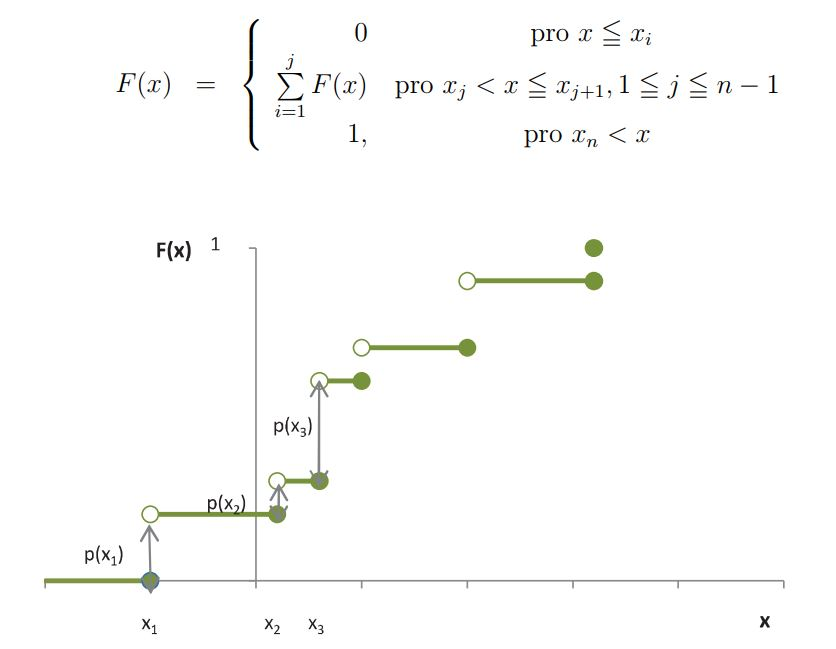
\includegraphics[width=0.6\textwidth]{assets/13_empiricka}
				\end{figure}
	\end{itemize}

	\item \textbf{Interkvartilové rozpětí IQR} -- Tato statistika je mírou variability souboru a je definována jako vzdálenost mezi horním a dolním kvartilem.
	\item \textbf{MAD} (median absolute deviation from the median) -- medián absolutních odchylek od mediánu 
			\begin{enumerate}
				\item Výběrový soubor uspořádáme podle velikosti.
				\item Určíme medián souboru.
				\item Pro každou hodnotu souboru určíme absolutní hodnotu její odchylky od mediánu.
				\item Absolutní odchylky od mediánu uspořádáme podle velikosti.
				\item Určíme medián absolutních odchylek od mediánu, tj. MAD.
			\end{enumerate}
	\item \textbf{Výběrový rozptyl} $\mathbf{s^2}$ (\uv{s kvadrát}, sample variance) --
		\begin{itemize}
			\item  je nejrozšířenější mírou variability výběrového souboru
			\begin{equation*}
				s^2 = \frac{\sum\limits_{i=1}^n (x_1 - \bar{x})^2} {n - 1}
			\end{equation*}
		\item Výběrový rozptyl je dán podílem součtu kvadrátu odchylek jednotlivých hodnot od průměru a rozsahu souboru sníženého o jedničku.
		\item Nevýhodou použití výběrového rozptylu jakožto míry variability je to, že jednotka této charakteristiky je druhou mocninou jednotky proměnné. Např. je--li proměnnou denní tržba uvedena v Kč, bude výběrový rozptyl této proměnné vyjádřen v Kč$^2$.
		\item Následující míra variability tuto vlastnost nemá.
	\end{itemize}
	\item \textbf{Výběrová směrodatná odchylka s} -- je definována jako kladná odmocnina výběrového rozptylu
	\begin{equation*}
				s = \sqrt{s^2} = \sqrt{\frac{\sum\limits_{i=1}^n (x_1 - \bar{x})^2} {n - 1}}.
	\end{equation*}
	Nevýhodou výběrového rozptylu i výběrové směrodatné odchylky je skutečnost, že neumožňují porovnávat varibilitu proměnných vyjádřených v různých jednotkách. Která proměnná má větší variabilitu – výška nebo hmotnost dospělého člověka? Na tuto otázku nám dá odpověď tzv. variační koeficient.
	\item \textbf{Variační koeficient} $\mathbf{V_x}$ -- vyjadřuje relativní míru variability proměnné x. Podle níže uvedeného vztahu jej lze stanovit pouze pro proměnné, které nabývají výhradně kladných hodnot. Variační koeficient je bezrozměrný. Uvádíme-li jej v [\%], hodnotu získanou z definičního vzorce vynásobíme 100\%.
	\begin{equation*}
				V_x = \frac{V}{\bar{x}}, popr. V_x = \frac{V}{\bar{x}} \cdot 100 [\%].
	\end{equation*}
\end{itemize}

\subsection{Identifikace odlehlých pozorování}
\begin{itemize}
	\item \textbf{Vnitřní hradby} -- Za odlehlé pozorování lze považovat takovou hodnotu $x_i$ , která je od dolního, resp. horního kvartilu vzdálená více než 1,5 násobek interkvartilového rozpětí. Tedy: $[(x_i < x_{0,25} - 1,5 \cdot IQR) \vee (x_i > x_{0,75} + 1,5 \cdot IQR)] \Rightarrow x_i$ je odlehlým pozorováním. 
	\item \textbf{z--souřadnice (z--skóre)} Za odlehlé pozorování lze považovat takovou hodnotu $x_i$, jejíž absolutní hodnota z-souřadnice je větší než 3, tj. hodnota, která je od průměru vzdálenější než 3s. Tedy: $z-skore_i = \frac{x_i - \bar{x}}{s}$ \\	
		$|z-skore_i| > 3 \Rightarrow |\frac{x_i - \bar{x}}{s}| >3s \Rightarrow x_i$ je odlehlým pozorováním.

	\item $\mathbf{x_{0,5}}$\textbf{--souřadnice ($\mathbf{x_{0,5}}$--skóre)} -- : Za odlehlé pozorování lze považovat takovou hodnotu $x_i$, jejíž absolutní hodnota mediánové souřadnice je větší než 3, tj. hodnota, která je od mediánu vzdálenější než $3 \cdot 1,483\cdot MAD$. Tedy: $x_{0,5}-skore_i = \frac{x_i - x_{0,5}}{1,483MAD}$ \\	
		$|x_{0,5}-skore_i| > 3 \Rightarrow |\frac{x_i - x_{0,5}}{1,483MAD}| >3 \Rightarrow |x_i - x_{0,5}| >3 \cdot 1,483MAD \Rightarrow x_i$ je odlehlým pozorováním.
\end{itemize}

\subsection{Míra šikmosti a špičatosti}	
 		\begin{itemize}
 			\item \textbf{Výběrová šikmost a} (skewness) -- vyjadřuje asymetrii rozložení hodnot proměnné kolem jejího průměru.
 				\begin{itemize}
 					\item $a = 0$ -- hodnoty proměnné jsou kolem jejího průměru rozloženy symetricky
					\item $a > 0$ -- u proměnné převažují hodnoty menší než průměr
					\item $a < 0$ -- u proměnné převažují hodnoty větší než průměr
				\begin{figure}[H]
				\centering
				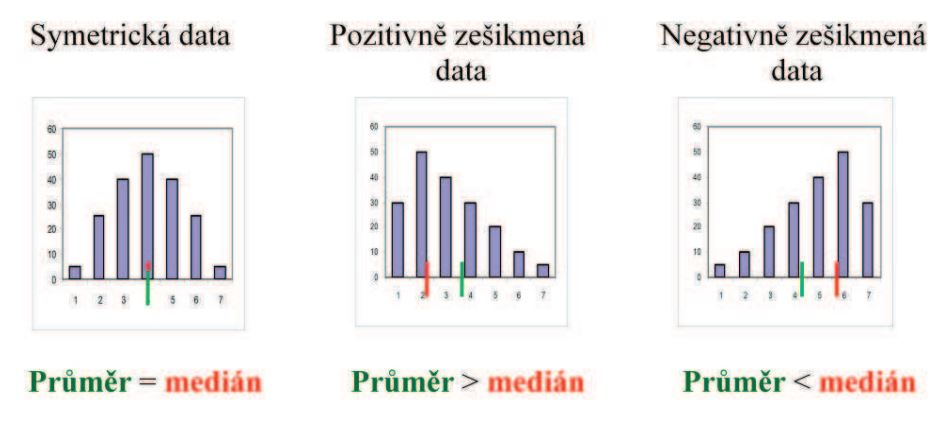
\includegraphics[width=0.6\textwidth]{assets/13_sikmost}
				\end{figure}
				\end{itemize}
				\item \textbf{Souvislost mezi šikmostí a charakteristikami polohy}
				\begin{itemize}
							\item Symetrické rozdělení: $\bar{x} = x_{0,5}$
							\item Pozitivně zešikmené rozdělení: $\bar{x} > x_{0,5}$
							\item Negativně zešikmené rozdělení: $\bar{x} < x_{0,5}$
				\end{itemize}
 			\item \textbf{Výběrová špičatost b} (kurtosis) -- vyjadřuje koncentraci hodnot proměnné kolem jejího průměru.
 				\begin{itemize}
 					\item $b = 0$ -- špičatost odpovídá normálnímu rozdělení (bude definováno později)
					\item $b > 0$ -- špičaté rozdělení proměnné
					\item $b < 0$ -- ploché rozdělení proměnné
				\begin{figure}[H]
				\centering
				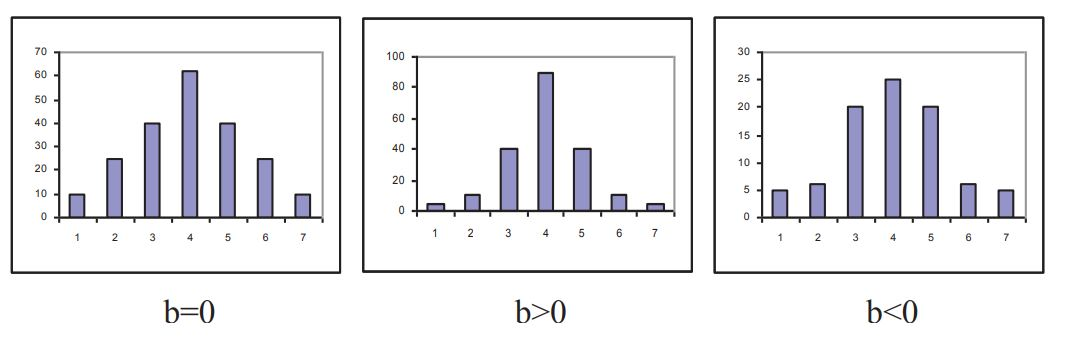
\includegraphics[width=0.6\textwidth]{assets/13_spicatost}
				\end{figure}
				\end{itemize}
 		\end{itemize}

\subsection{Grafické znázornění kvalitativní proměnné}
\begin{itemize}
	\item \textbf{Krabicový graf} (Box plot)
	\begin{itemize}
		\item Odlehlá pozorování jsou znázorněna jako izolované body, konec horního (popř. konec dolního) vousu představují maximum (popř. minimum) proměnné po vyloučení odlehlých pozorování,\uv{víko} krabice udává horní kvartil, \uv{dno} dolní kvartil, vodorovná úsečka uvnitř krabice označuje medián.
		\item Z polohy mediánu vzhledem ke \uv{krabici} lze dobře usuzovat na symetrii vnitřních 50\% dat a my tak získáváme dobrý přehled o středu a rozptýlenosti proměnné.
	\end{itemize}
				\begin{figure}[H]
				\centering
				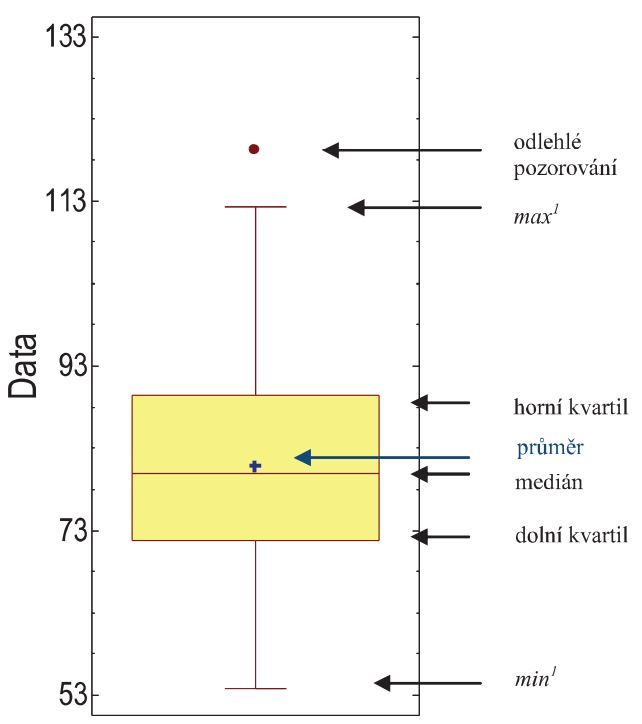
\includegraphics[width=0.5\textwidth]{assets/13_box_plot}
				\end{figure}
	\item \textbf{Číslicový histogram} (Lodyha s listy, angl. Stem and leaf plot)
	\begin{itemize}
		\item Jak jsme si ukázali, výhodou krabicového grafu je jeho jednoduchost, někdy nám však chybí informace o konkrétních hodnotách proměnné. 
		\item Chtěli bychom proto nějak přehledně zapsat číselné hodnoty výběru a k tomu nám slouží právě číslicový histogram.
		\item Navíc nám tento graf dává dobrou představu o šikmosti proměnné.
		\item Příklad: \textit{Představme si proměnnou představující průměrné měsíční platy zaměstnanců ve státní správě}.
		\begin{table}[H]
	\centering
	\begin{tabular}{|l|}
		\hline
		\textbf{Průměrný měsíční plat [Kč]}                                \\ \hline
		10 654, 9 765, 8 675, 12 435, 9 675, 10 343, 18 786, 15 420, 8 675,	7 132, \\
		6 732,6 878, 15 657, 9 754, 9 543, 9 435, 10 647, 12 453, 9 987, 10 342.                                                                 \\ \hline

	\end{tabular}
\end{table}
				\begin{figure}[H]
				\centering
				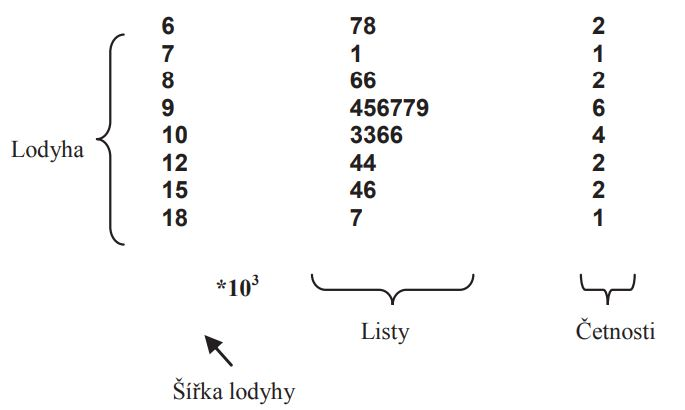
\includegraphics[width=0.6\textwidth]{assets/13_cislicovy_hist}
				\end{figure}
		\begin{itemize}
		 \item Pro naší informaci nejsou tak důležité koruny ani desetikoruny rozdílu. V tomto případě se nám jedná přinejmenším o stokoruny.
		 \item Co kdybychom tedy informaci o \uv{nedůležitých} řádech zanedbali a znázornili setříděná data pouze na základě vyšších řádů? My jsme se rozhodli, že důležitý řád jsou pro nás stokoruny.
		 \item Hodnoty stojící o řád výš (v našem případě tisíce) zapíšeme setříděné pod sebe, tak, že tvoří jakýsi stonek (\textbf{lodyhu}), přičemž pod graf uvedeme tzv. \textbf{šířku lodyhy}, která udává koeficient, jímž se hodnoty uvedené v grafu násobí.
		 \item Druhý sloupec grafu, \textbf{listy}, budou tvořit číslice, reprezentujíci zvolený \uv{důležitý} řád, zapisované do příslušných řádků (opět seřazené podle velikosti).
		 \item Třetí sloupec udává absolutní četnosti příslušné daným řádkům.
		\end{itemize}
	\end{itemize}
\end{itemize}

\subsection{Statistické charakteristiky kvalitativních proměnných}
\subsubsection{Nominální proměnná}
Nominální proměnná nabývá v rámci souboru různých, avšak rovnocenných kategorií. Počet těchto kategorií nebývá příliš vysoký, a proto první statistickou charakteristikou, kterou k popisu proměnné použijeme je četnost.
\begin{itemize}
	\item \textbf{Četnost} $\mathbf{n_i}$ (absolutní četnost, \uv{frequency}) --  je definována jako počet výskytu dané varianty kvalitativní proměnné. V případě, že kvalitativní proměnná ve statistickém souboru o rozsahu $n$ hodnot  nabývá $k$ různých variant, jejichž četnosti označíme $n_1, n_2, ... , n_k$, musí zřejmě platit $n_1 + n_2 + ... + n_k = \sum\limits_{i=1}^k n_i = n$. \\
	Chceme-li vyjádřit, jakou část souboru tvoří proměnné s některou variantou, použijeme pro popis proměnné relativní četnost.

	\item \textbf{Relativní četnost} $\mathbf{p_i}$ (\uv{relative frequency}) je definována jako $p_i = \frac{n_i}{n}$, popř. $p_i = \frac{n_i}{n} \cdot 100 [\%]$. Pro relativní četnosti musí platit $p_1 + p_2 + ... + p_k = \sum\limits_{i=1}^k p_i = p$. \\
	Při zpracování kvalitativní proměnné je vhodné četnosti i relativní četnosti uspořádat do tzv. \textbf{tabulky rozdělení četnosti} (\uv{frequency table})
				\begin{figure}[H]
				\centering
				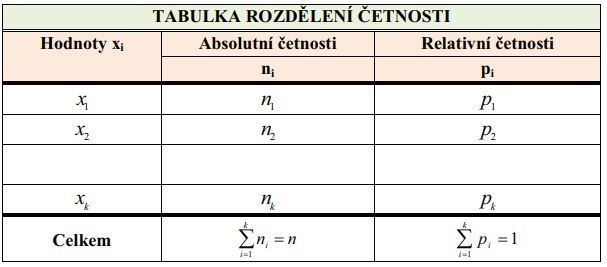
\includegraphics[width=0.6\textwidth]{assets/13_tabl_cetnost}
				\end{figure}
	\item \textbf{Modus} -- s definujeme jako název varianty proměnné vykazující nejvyšší četnost.\\
	\item \textbf{Grafické znázornění nominální proměnné} 
	\begin{itemize}
		\item \textbf{Histogram} -- je klasickým grafem, v němž na jednu osu vynášíme varianty proměnné a na druhou osu jejich četnosti. Jednotlivé hodnoty četností jsou pak zobrazeny jako výšky sloupců (obdélníků, popř. hranolů, kuželů...)
		\item \textbf{Výsečový graf} -- prezentuje relativní četnosti jednotlivých variant proměnné, přičemž jednotlivé relativní četnosti jsou úměrně reprezentovány plochami příslušných kruhových výsečí. (Změnou kruhu na elipsu dojde k trojrozměrnému efektu.)
	\end{itemize}
\end{itemize}
\subsubsection{Ordinální proměnná}
Ordinální proměnná, stejně jako proměnná nominální, nabývá v rámci souboru různých slovních variant, avšak tyto varianty mají přirozené uspořádání, tj. můžeme určit, která je \uv{menší} a která \uv{větší}. 
\begin{itemize}
	\item \textbf{Kumulativní četnost} $\mathbf{m_i}$ i (\uv{cumulative frequency}) -- definujeme jako počet hodnot proměnné, které nabývají varianty nižší nebo rovné i-té variantě. \\ 
	\textit{Uvažte např. proměnnou \uv{známka ze statistiky}, která nabývá variant: \uv{výborně}, \uv{velmi dobře}, \uv{prospěl}, \uv{neprospěl}, pak např. kumulativní četnost pro variantu \uv{prospěl} bude rovna počtu studentů, kteří ze statistiky získali známku \uv{prospěl} nebo lepší.} \\
	Jsou-li jednotlivé varianty uspořádány podle své \uv{velikosti}(\uv{$x_1 < x_2 < ... < x_k$}), platí $m_i = \sum\limits_{i=1}^i n_j$, Je tedy zřejmé, že kumulativní četnost $k$--té (\uv{nejvyšší}) varianty je rovna rozsahu proměnné $– mk = n$.

	\item \textbf{Kumulativní relativní četnost} $\mathbf{F_i}$ (\uv{cumulative relative frequency}) -- vyjadřuje jakou část souboru tvoří hodnoty nabývající i-té a nižší varianty. $F_i = \sum\limits_{j=1}^i p_j,$ což není nic jiného než relativní vyjádření kumulativní četnosti: $F_i = \frac{m_i}{n}$. \\ 
	Obdobně jako pro nominální proměnné, můžeme i pro proměnné ordinální prezentovat statistické charakteristiky pomocí tabulky rozdělení četnosti. Ta obsahuje ve srovnání s tabulkou rozdělení četností pro nominální proměnnou navíc hodnoty kumulativních a kumulativních relativních četností.\\
				\begin{figure}[H]
				\centering
				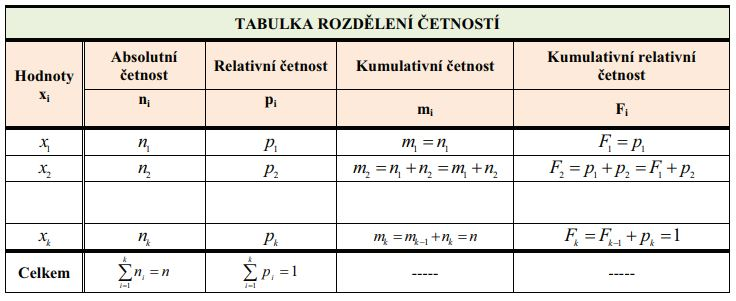
\includegraphics[width=0.8\textwidth]{assets/13_tabl_cetnost_ord}
				\end{figure}
	\item \textbf{Grafické znázornění ordinální proměnné}
	\begin{itemize}
		\item \textbf{Lorenzova křivka} ((polygon kumulativních četností, Galtonova ogiva, S křivka) -- S křivka) je spojnicovým grafem, který získáme tak, že na vodorovnou osu vynášíme jednotlivé varianty proměnné v pořadí od \uv{nejmenší} do \uv{největší} a na svislou osu příslušné hodnoty kumulativních četností. Znázorněné body spojíme úsečkami.
				\begin{figure}[H]
				\centering
				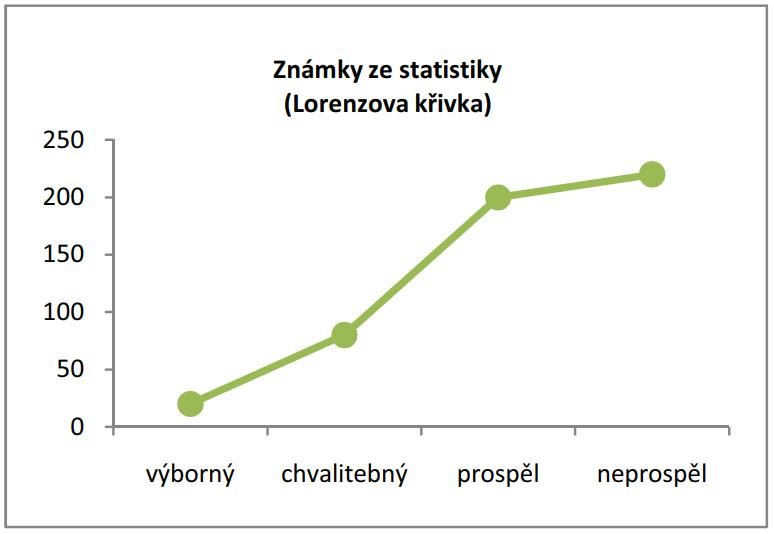
\includegraphics[width=0.5\textwidth]{assets/13_lorenzo}
				\end{figure}
		\item \textbf{Paretova analýza} -- lze formulovat tak, že 80\% následků pramení z 20\% příčin (20\% lidí vlastní 80\% celkového bohatství). V praxi pak bývá snahou nalézt toto malé spektrum příčin (životně důležitá menšina), které tak významně ovlivňuje výsledek.
	\end{itemize}
\end{itemize}
